\documentclass[10pt]{beamer}

\usepackage{fontspec}
\usetheme{metropolis}

\usepackage{booktabs}
\usepackage[scale=2]{ccicons}

\usepackage{pgfplots}
\usepgfplotslibrary{dateplot}

\usepackage{xspace}
\newcommand{\themename}{\textbf{\textsc{metropolis}}\xspace}

\usepackage{listings}
\usepackage{xcolor}
\usepackage{lmodern}

\lstset{
	basicstyle=\ttfamily,
	frame=shadowbox,
	rulesepcolor=\color{gray},
	columns=fullflexible,
	commentstyle=\color{gray},
	keywordstyle=\bfseries\color{red},
	escapeinside={\%*}{*)},
  aboveskip=2em,
  captionpos=b,
  abovecaptionskip=1em,
  belowcaptionskip=1em
}

\title{Midway presentation}
\subtitle{Group 1}
\date{12 November 2018}
\author{Claudio Maggioni}
\titlegraphic{\centering{
\includegraphics[height=1.5cm]{logo.png}}}

\begin{document}

\maketitle

\begin{frame}[standout]
\centering{\Huge\LaTeX}
\end{frame}

\section{Progress up to now}

\begin{frame}[fragile]{Search box}
\vfill\centering{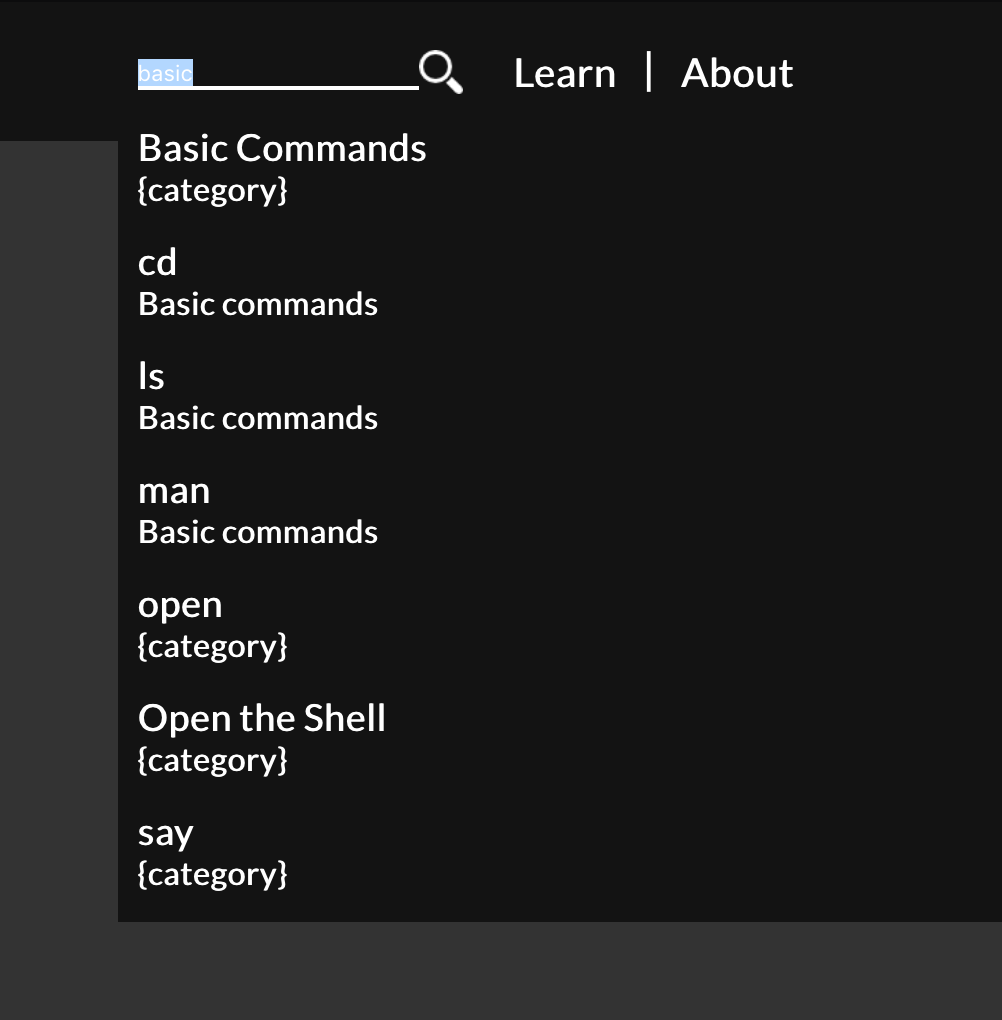
\includegraphics[width=0.6\textwidth]{search.png}}\vfill
\end{frame}

\begin{frame}[fragile]{Automatic topic index pages}
\vfill\centering{
\includegraphics[width=0.6\textwidth]{index.png}}\vfill
\end{frame}

\begin{frame}[fragile]{Basic style}
\vfill\centering{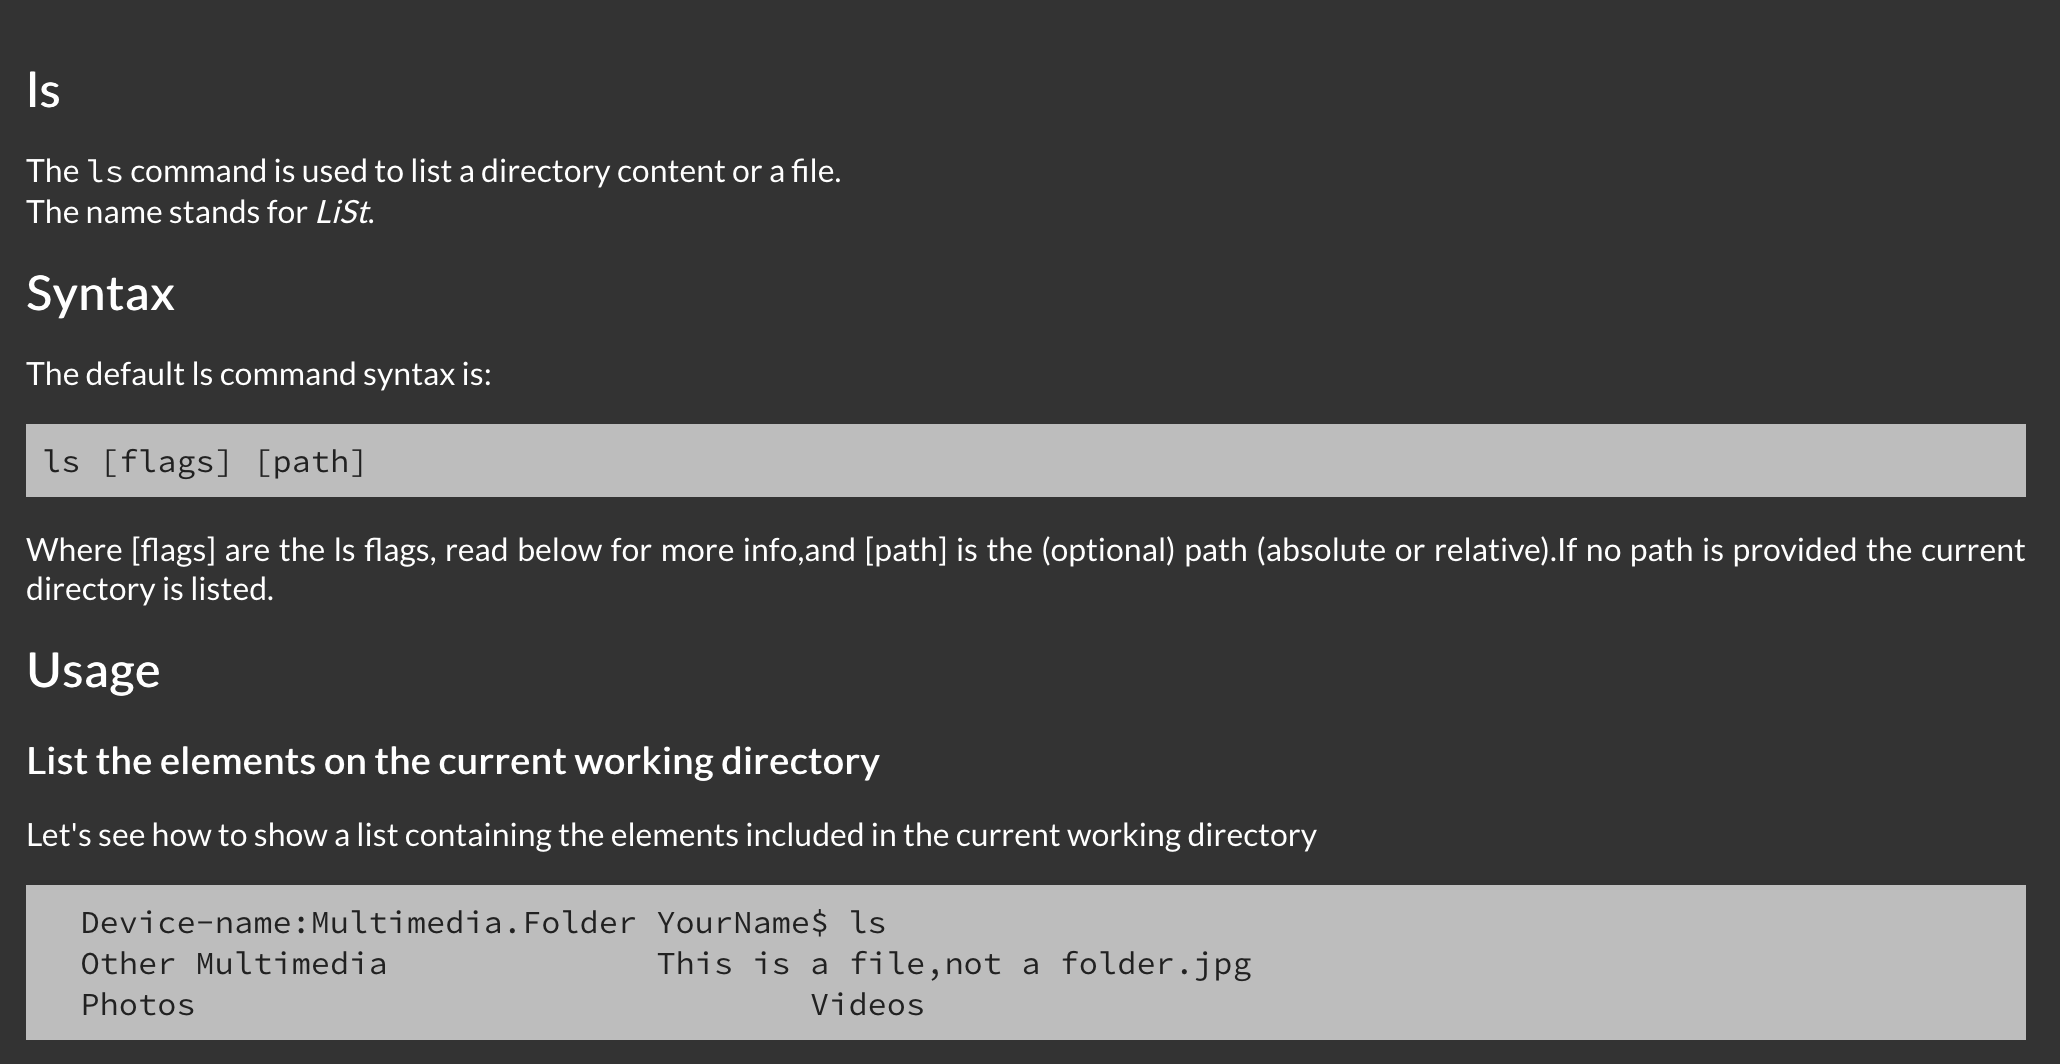
\includegraphics[width=\textwidth]{formatting.png}}\vfill
\end{frame}

\begin{frame}[fragile]{Automatic attribution in footer}
\vfill\centering{
\includegraphics[width=0.8\textwidth]{footer.png}}\vfill
\end{frame}

\section{First code review for content}

{\setbeamercolor{background canvas}{bg=black}
\begin{frame}
\centering{\Huge\fontspec{Comic Sans MS}\color{red} 
	\textsc{The evil side of HTML \\
	\vspace{0.5cm}
	(and Jekyll)}}
\end{frame}}

\begin{frame}[fragile]
\begin{figure}[h]
\begin{lstlisting}[language=html]
title: ...
...
---

<html>
<head>
</head>

<body>
<header>

<h1>...</h1>
...
</header>
</body>
</html>
\end{lstlisting}
\end{figure}
\end{frame}

\begin{frame}[fragile]
\begin{figure}[h]
\begin{lstlisting}[language=html]
<div class="title1">
    <h1>...</h1>
</div>

A list of things:
<br> ...
<br> ...
<br> ...
<br> ...
<br> ...
\end{lstlisting}
\end{figure}
\end{frame}

\begin{frame}[fragile]
\begin{figure}[h]
\begin{lstlisting}[language=html]
<!-- No Jekyll header -->

<!DOCTYPE html>
...
\end{lstlisting}
\end{figure}
\end{frame}

\begin{frame}{Page creation guide}
\vfill\centering{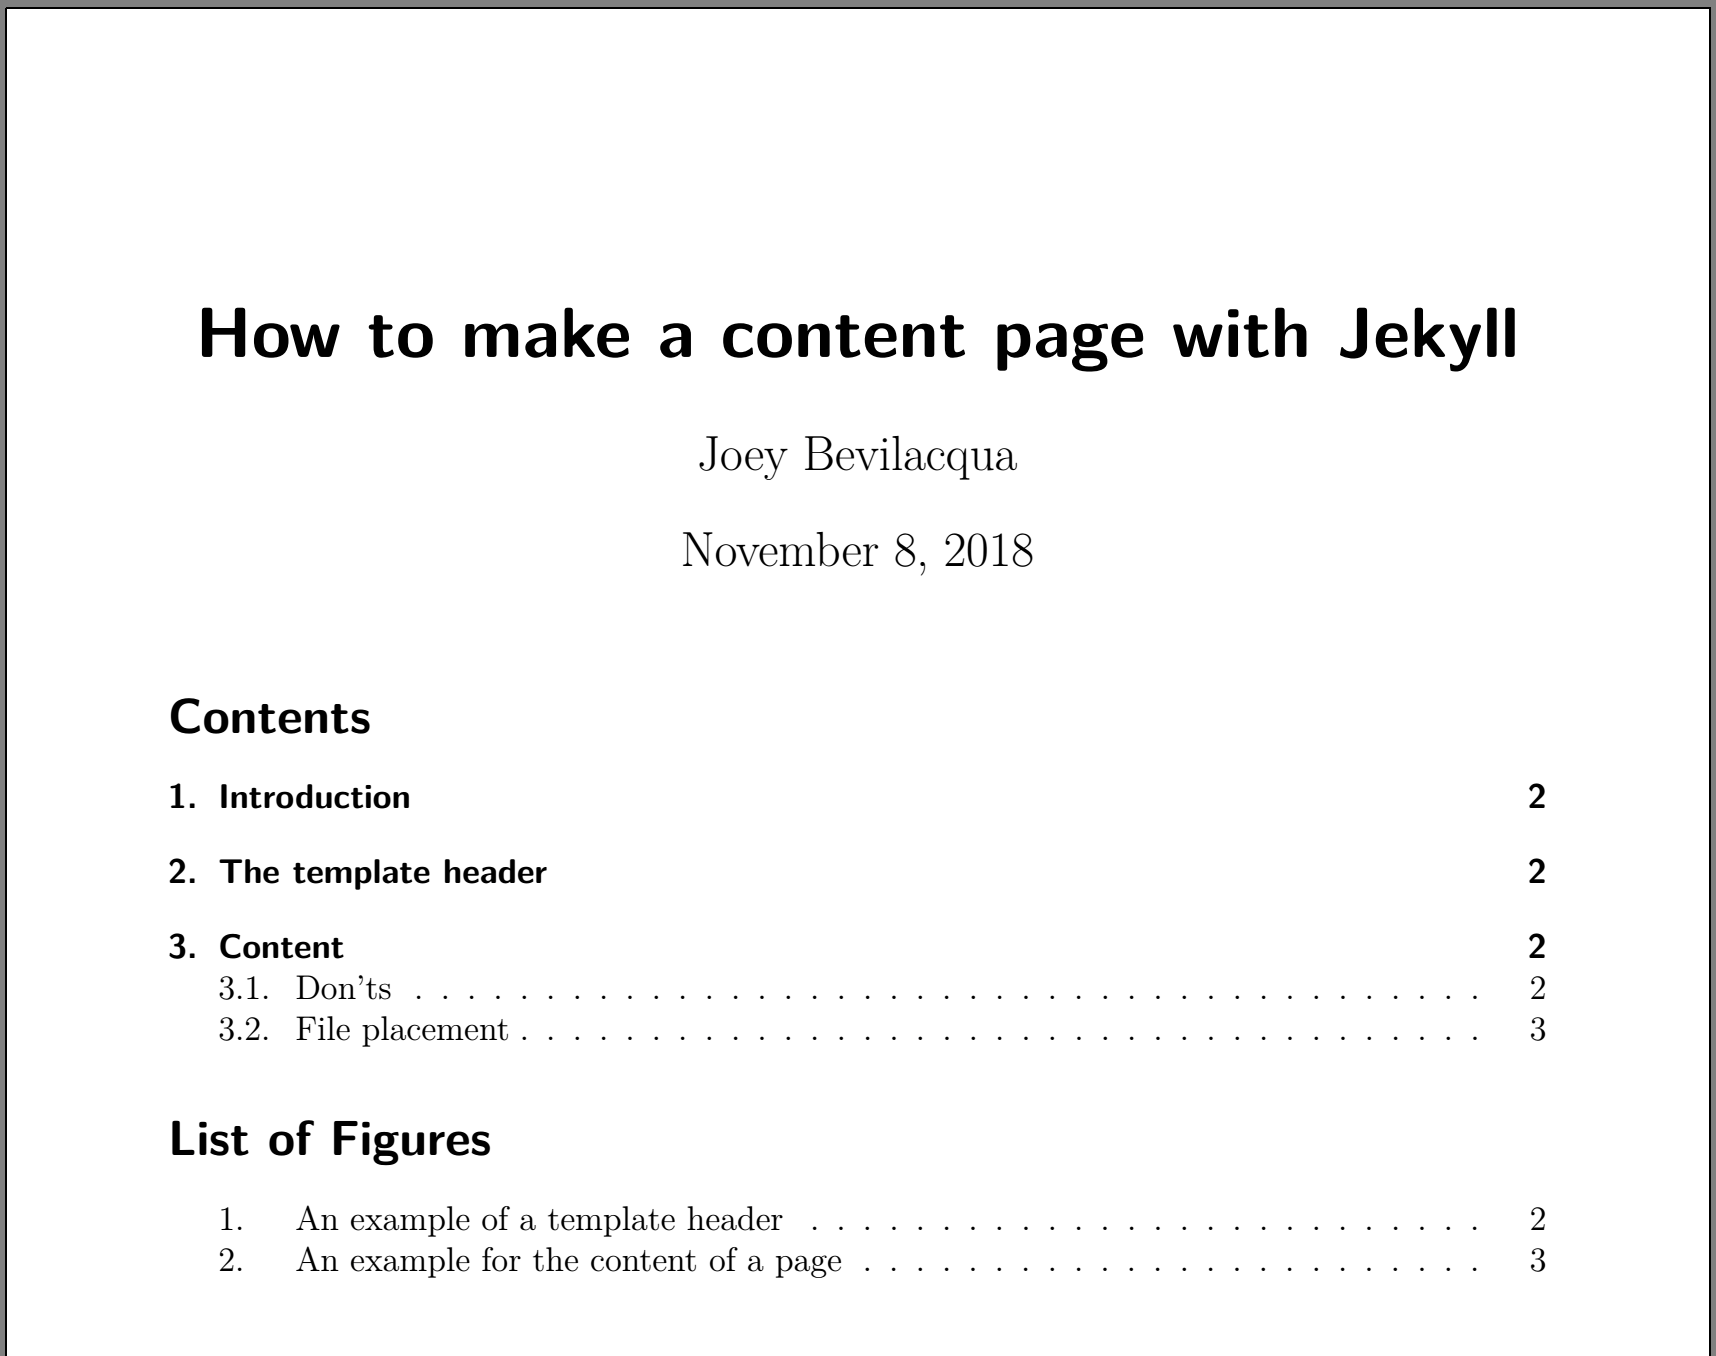
\includegraphics[width=0.8\textwidth]{page_creation.png}}\vfill
\end{frame}

\section{Code contribution of each team}

\begin{frame}{Code contribution of each team}
\begin{figure}
    \begin{tikzpicture}
      \begin{axis}[
        legend pos=north west,
        mbarplot,
        ylabel={Bar},
        enlarge x limits={0.5},
        symbolic x coords={a small bar,a medium bar,a large bar},
        width=\textwidth,
        height=6cm,
        xtick=data
      ]
      
      \legend{FS, Front, Basic, Interm, Advanced, Scripting}

      \addplot plot coordinates {(a small bar,42)
        (a medium bar,50)
        (a large bar,60)};
      \addplot plot coordinates {(a small bar,42)
        (a medium bar,50)
        (a large bar,60) };
      \addplot plot coordinates {(a small bar,42)
        (a medium bar,50)
        (a large bar,60)};
      \addplot plot coordinates {(a small bar,42)
        (a medium bar,50)
        (a large bar,60)};
      \addplot plot coordinates {(a small bar,42)
        (a medium bar,50)
        (a large bar,60)};
      \addplot plot coordinates {(a small bar,42)
        (a medium bar,50)
        (a large bar,60)};
      \end{axis}
    \end{tikzpicture}
  \end{figure}
\end{frame}

\end{document}
